\documentclass[a4paper]{article}

\usepackage{fancyhdr}
\usepackage{color}
\usepackage{listings}
\usepackage{amsmath}
\usepackage{amsthm}
\usepackage{amsfonts}
\usepackage{graphicx}
\usepackage{float}
\usepackage{tikz}

%\usepackage{tilings}

\usetikzlibrary{graphs}
\usetikzlibrary{graphs.standard}

\usepackage[hmargin=3cm,vmargin=3.5cm]{geometry}

\newtheorem{lemma}{Lemma}
\newtheorem{theorem}{Theorem}
\newtheorem{definition}{Definition}
\newtheorem*{definition*}{Definition}
\newtheorem{conjecture}{Conjecture}
\newtheorem{corollary}{Corollary}

\newcommand{\R}{\text{Re}}
\newcommand{\I}{\text{Im}}
\newcommand{\Arg}{\text{Arg}}
\newcommand{\dist}{\text{d}}

\pagenumbering{arabic}
\pagestyle{fancyplain}

\fancyhf{}
\lhead[Wiener Index Families]{Wiener Index Families}
%\rhead[Notes]{Notes}
\cfoot[\thepage]{\thepage}


\begin{document}

The tiling of the plane by six cycles, as in the following image.



%square tiling
\begin{center}
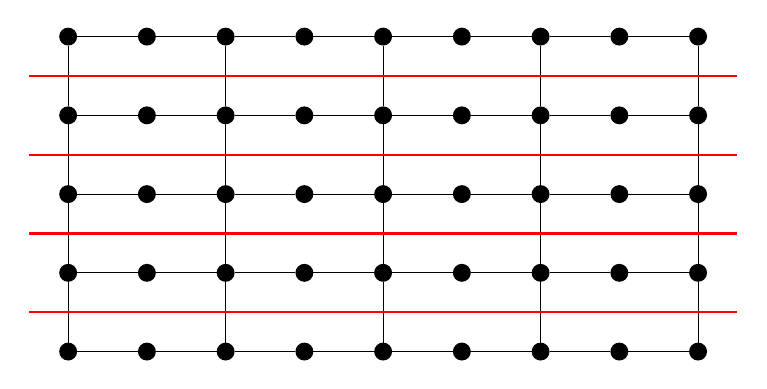
\begin{tikzpicture}[every node/.style={draw,circle,thick,fill=black,inner sep=2pt}]
\def\size{4}
\pgfmathparse{(2*\size)+1}
\xdef\hori{\pgfmathresult}
\pgfmathparse{\size + 1}
\xdef\vertical{\pgfmathresult}

%graph

%vertices
\foreach \x in {1,...,\hori}
	\foreach \y in {1,...,\vertical}
	\node (\x\y) at (\x,\y) {};
	
%edges
%horizontal
\pgfmathparse{\hori-1}
\xdef\horiz{\pgfmathresult}
\foreach \x in {1,...,\horiz}
	\foreach \y in {1,...,\vertical}
	{\pgfmathsetmacro{\next}{int(\x + 1)}
	\draw (\x\y) -- (\next\y);}

%vertical
\pgfmathparse{\vertical-1}
\foreach \x in {1,3,...,\hori}
\foreach \y in {1,...,\pgfmathresult}
	{\pgfmathsetmacro{\next}{int(\y + 1)}
	\draw (\x\y) -- (\x\next);}
	
%cuts

%horizontal
\pgfmathparse{\hori+0.5}
\xdef\cutwidth{\pgfmathresult}
\foreach \x in {1,...,\size}
	\foreach \y in {1,...,\size}
		\draw [red,thick]  (\x-0.5,\y+0.5) -- (\cutwidth,\y+0.5);
		
%vertical
\end{tikzpicture}
\end{center}

\vspace{10mm}

To calculate the Wiener index, we need to consider three different cut families, the horizontal cuts, and two families of vertical cuts, which are identical, so only one of them needs to be considered, and then in the the final calculation, counted twice.

The following image is a different tiling of the plane with six cycles, often called a parquetry tiling.
%parquetry
\begin{center}
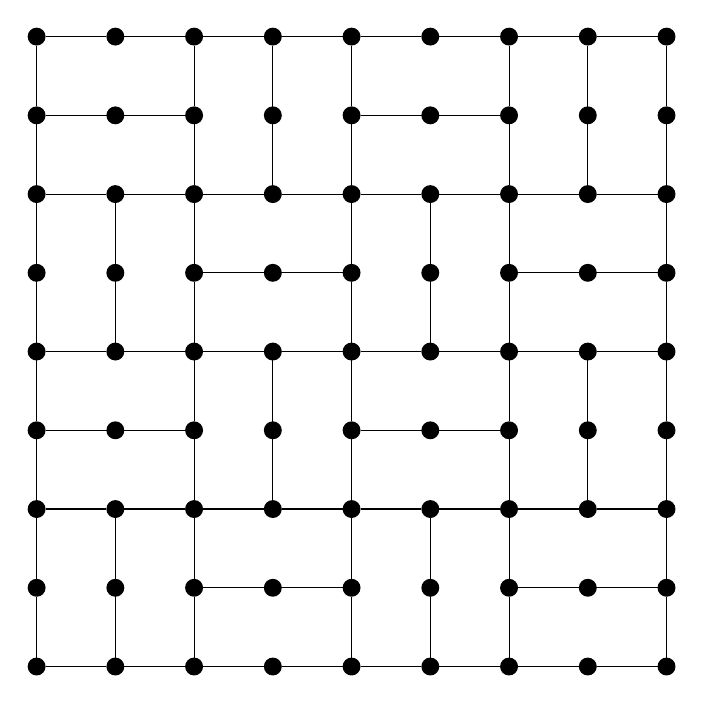
\begin{tikzpicture}[every node/.style={draw,circle,thick,fill=black,inner sep=2pt}]
\def\size{2}
\pgfmathparse{int(4*\size+1)}
\xdef\horizontal{\pgfmathresult}
\pgfmathparse{int(4*\size + 1)}
\xdef\vertical{\pgfmathresult}
\pgfmathparse{\horizontal-1}
\xdef\hori{\pgfmathresult}
\pgfmathparse{\vertical-1}
\xdef\vert{\pgfmathresult}

%graph

%vertices
\foreach \x in {1,...,\horizontal}
	\foreach \y in {1,...,\vertical}
	\node (\x a\y) at (\x,\y) {};
	
%edges
%fixed edges
\foreach \x in {1,...,\hori}
	\foreach \y in {1,3,...,\vertical}
	{\pgfmathsetmacro{\next}{int(\x+1)}
	\draw (\x a\y)--(\next a\y);}

\foreach \y in {1,...,\vert}
	\foreach \x in {1,3,...,\horizontal}
	{\pgfmathsetmacro{\next}{int(\y+1)}
	\draw (\x a\y)--(\x a\next);}
	
%horizontal edges
\foreach \x in {1,5,...,\hori}
	\foreach \y in {1,...,\vertical}{
	\pgfmathparse{Mod(\y,4)==0?1:0}
	\ifnum\pgfmathresult>0{
		\pgfmathsetmacro{\next}{int(\x+2)}
		\draw (\x a\y) -- (\next a\y);}
	\else {}
	\fi}

\foreach \x in {3,7,...,\hori}
	\foreach \y in {1,...,\vertical}{
	\pgfmathparse{Mod(\y,4)==2?1:0}
	\ifnum\pgfmathresult>0{
		\pgfmathsetmacro{\next}{int(\x+2)}
		\draw (\x a\y) -- (\next a\y);}
	\else {}
	\fi}
	
%vertical edges
\foreach \y in {1,5,...,\vert}
	\foreach \x in {1,...,\horizontal}{
	\pgfmathparse{Mod(\x,4)==2?1:0}
	\ifnum\pgfmathresult>0{
		\pgfmathsetmacro{\next}{int(\y+2)}
		\draw (\x a\y) -- (\x a\next);}
	\else {}
	\fi}
	
\foreach \y in {3,7,...,\vert}
	\foreach \x in {1,...,\horizontal}{
	\pgfmathparse{Mod(\x,4)==0?1:0}
	\ifnum\pgfmathresult>0{
		\pgfmathsetmacro{\next}{int(\y+2)}
		\draw(\x a\y) -- (\x a\next);}
	\else {}
	\fi}
\end{tikzpicture}
\end{center}

There is only one family of cuts that need to be considered for the parquetry tiling due to it having rotation symmetry. In the final calculation we simply multiple the number obtained from this single family by four to get the Wiener index.

\newpage

The top half of an aztec diamond, picture below.
%half aztec diamond
\begin{center}
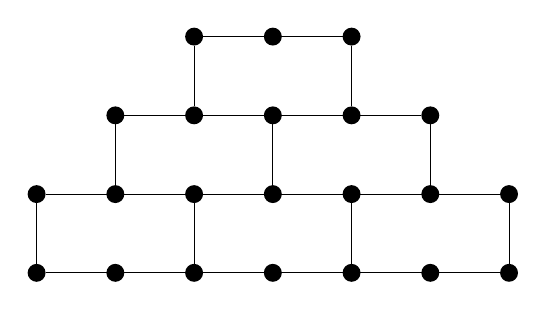
\begin{tikzpicture}[every node/.style={draw,circle,thick,fill=black,inner sep=2pt}]
\def\size{3}
\xdef\horizontal{3}
\pgfmathparse{\size + 1}
\xdef\vertical{\pgfmathresult}

%vertices
\xdef\k{\size}
\foreach \y in {\size,...,1}{
	\foreach \x in {1,...,\horizontal}{
		\pgfmathsetmacro{\pos}{int(\x+\k)}
		\node (\x a\y) at (\pos,\y) {};}
	\pgfmathparse{int(\horizontal+2)}
	\xdef\horizontal{\pgfmathresult}
	\pgfmathparse{int(\k-1)}
	\xdef\k{\pgfmathresult}
}

\pgfmathparse{int(\horizontal-2)}
\xdef\horizontal{\pgfmathresult}
\foreach \x in {1,...,\horizontal} {
	\pgfmathsetmacro{\pos}{int(\x + 1)}
	\node (\x a0) at (\pos,0) {};}


%edges
%horizontal
\xdef\horizontal{3}
\foreach \y in {\size,...,1}{
	\draw (1a\y)--(\horizontal a\y);
	\pgfmathparse{int(\horizontal+2)}
	\xdef\horizontal{\pgfmathresult}
}
\pgfmathparse{int(\horizontal - 2)}
\xdef\horizontal{\pgfmathresult}
\draw (1a0) -- (\horizontal a0);

%vertical
\xdef\horizontal{5}
\pgfmathparse{int(\size - 1)}
\xdef\s{\pgfmathresult}
\foreach \y in {\s,...,2} {
	\xdef\k{2}
	\foreach \x in {1,3,...,\horizontal} {
		\pgfmathsetmacro{\next}{int(\y-1)}
		\draw (\x a\y) -- (\k a\next);
		\pgfmathparse{int(\k+2)}
		\xdef\k{\pgfmathresult}}
	\pgfmathparse{int(\horizontal+2)}
	\xdef\horizontal{\pgfmathresult}
}
\foreach \x in {1,3}{
	\pgfmathsetmacro{\next}{int(\size-1)}
	\pgfmathsetmacro{\xr}{int(\x+1)}
	\draw (\x a\size) -- (\xr a\next);
}
\pgfmathparse{2*\size+1}
\xdef\horizontal{\pgfmathresult}
\foreach \x in {1,3,...,\horizontal}
	\draw (\x a1) -- (\x a0);
\end{tikzpicture}
\end{center}

There are three cut families to consider with this graph. It is not obvious from this diagram, but all three families are the same, so again, we only need to calculate the value for one family, and multiple by three.

\vspace{10mm}

The Aztec diamond, picture below.
%Aztec diamond
\begin{center}
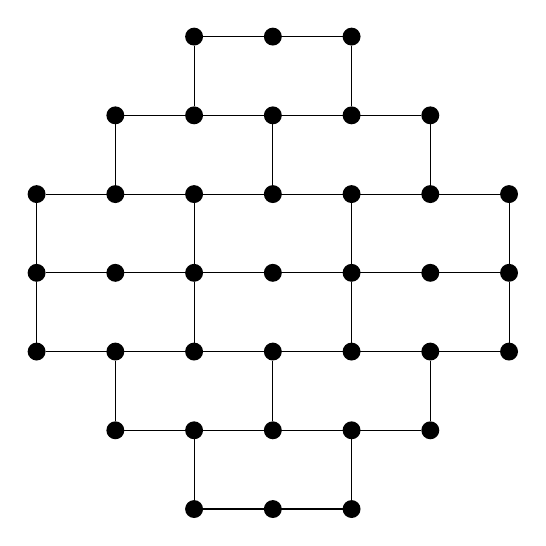
\begin{tikzpicture}[every node/.style={draw,circle,thick,fill=black,inner sep=2pt}]
\def\size{3}
\xdef\horizontal{3}
\pgfmathparse{2*\size+1}
\xdef\vertical{\pgfmathresult}

%vertices
\xdef\k{\size}
\foreach \y in {\size,...,1}{
	\foreach \x in {1,...,\horizontal} {
		\pgfmathsetmacro{\pos}{int(\x+\k)}
		\node (\x a\y) at (\pos,\y) {};}
	\pgfmathparse{int(\horizontal+2)}
	\xdef\horizontal{\pgfmathresult}
	\pgfmathparse{int(\k-1)}
	\xdef\k{\pgfmathresult}
}

\pgfmathparse{int(\horizontal-2)}
\xdef\horizontal{\pgfmathresult}
\foreach \x in {1,...,\horizontal} {
	\pgfmathsetmacro{\pos}{int(\x + 1)}
	\node (\x a0) at (\pos,0) {};
}

\xdef\k{1}
\foreach \y in {-1,...,-\size}{
	\foreach \x in {1,...,\horizontal} {
		\pgfmathsetmacro{\pos}{int(\x+\k)}
		\node (\x a\y) at (\pos,\y) {};}
	\pgfmathparse{int(\horizontal-2)}
	\xdef\horizontal{\pgfmathresult}
	\pgfmathparse{int(\k+1)}
	\xdef\k{\pgfmathresult}
}

%edges
%horizontal
\xdef\horizontal{3}
\foreach \y in {\size,...,1}{
	\draw (1a\y)--(\horizontal a\y);
	\pgfmathparse{int(\horizontal+2)}
	\xdef\horizontal{\pgfmathresult}
}
\pgfmathparse{int(\horizontal -2)}
\xdef\horizontal{\pgfmathresult}
\draw (1a0) -- (\horizontal a0);
\foreach \y in {-1,...,-\size} {
	\draw (1a\y)--(\horizontal a\y);
	\pgfmathparse{int(\horizontal-2)}
	\xdef\horizontal{\pgfmathresult}
}

%vertical
\xdef\horizontal{5}
\pgfmathparse{int(\size-1)}
\xdef\s{\pgfmathresult}
\foreach \y in {\s,...,2} {
	\xdef\k{2}
	\foreach \x in {1,3,...,\horizontal} {
		\pgfmathsetmacro{\next}{int(\y-1)}
		\draw (\x a\y) -- (\k a\next);
		\draw (\x a-\y) -- (\k a-\next);
		\pgfmathparse{int(\k+2)}
		\xdef\k{\pgfmathresult}}
	\pgfmathparse{int(\horizontal+2)}
	\xdef\horizontal{\pgfmathresult}
}

\foreach \x in {1,3}{
	\pgfmathsetmacro{\next}{int(\size-1)}
	\pgfmathsetmacro{\xr}{int(\x+1)}
	\draw (\x a\size) -- (\xr a\next);
	\draw (\x a-\size) -- (\xr a-\next);
}
\pgfmathparse{2*\size+1}
\xdef\horizontal{\pgfmathresult}
\foreach \x in {1,3,...,\horizontal}{
	\draw (\x a1) -- (\x a0);
	\draw (\x a-1) -- (\x a0);
}

\end{tikzpicture}
\end{center}

The Aztec diamond has three families, the horizontal family, and two vertical families, which once again are symmetric, so only need to be calculated once, and counted twice in the evaluation of the Wiener index.
\end{document}